\documentclass[11pt,a4paper]{article}

\usepackage[margin=1in]{geometry}
\usepackage[hidelinks]{hyperref}
\usepackage{booktabs}
\usepackage{listings}
\usepackage{xcolor}
\usepackage{tikz}
\usepackage{graphicx}
\usepackage{float}
\usetikzlibrary{arrows.meta,positioning,shapes.geometric,fit,calc}

\title{FlexQL --- Design Document}
\author{<Name> \; <Roll No>}
\date{\today}

\definecolor{codebg}{RGB}{248,248,248}
\lstset{
  basicstyle=\ttfamily\small,
  breaklines=true,
  frame=single,
  backgroundcolor=\color{codebg},
  columns=fullflexible
}

\begin{document}
\maketitle
\tableofcontents
\newpage

\section{Overview}
FlexQL is a client--server relational database implemented in C11. The system exposes a small SQL subset through a C client API. The server executes statements against an in-memory row store for performance and optionally persists all mutations to a disk-backed Write-Ahead Log (WAL) for durability and crash recovery.

\subsection{Goals}
\begin{itemize}
  \item Provide a simple SQL server with a clean C client API.
  \item Support high insert throughput for large workloads (e.g., 10 million rows) via batching.
  \item Support concurrency: multiple clients and parallel query execution.
  \item Support optional persistence and fault tolerance using WAL replay.
\end{itemize}

\subsection{Non-goals / out of scope}
\begin{itemize}
  \item Full SQL compatibility.
  \item Advanced query planner/optimizer.
  \item UPDATE/DELETE, complex WHERE with AND/OR (if not implemented).
  \item SHOW TABLES / SHOW DATABASES (not implemented).
\end{itemize}

\section{Repository Layout}
Key paths:
\begin{itemize}
  \item \texttt{src/server/server.c}: server accept loop + batch protocol handling
  \item \texttt{src/network/net.c}: framed TCP send/recv, batched writev helpers
  \item \texttt{src/parser/parser.c}: SQL tokenizer + fast multi-row INSERT parser
  \item \texttt{src/query/executor.c}: statement execution entry point
  \item \texttt{src/storage/storage.c}: table/row storage, arenas, TTL sweeper integration
  \item \texttt{src/storage/persistence.c}: WAL background writer + startup replay
  \item \texttt{src/index/index.c}: open-addressing hash index
  \item \texttt{src/cache/cache.c}: LRU query cache
  \item \texttt{src/concurrency/threadpool.c}: fixed worker thread pool
  \item \texttt{src/client/client.c}: libflexql API + REPL client
\end{itemize}

\section{System Architecture}
FlexQL follows a classic client--server model over TCP.

\begin{figure}[H]
\centering
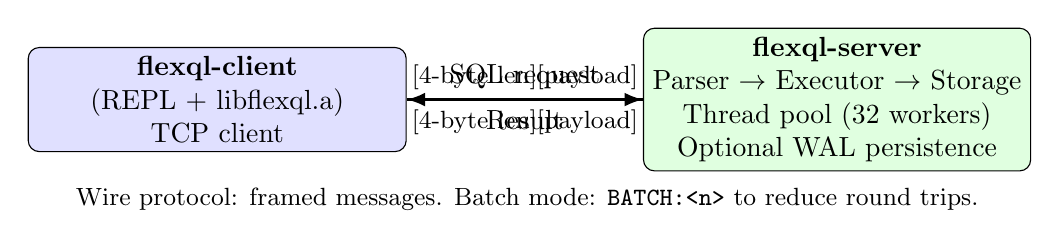
\begin{tikzpicture}[
  box/.style={rectangle,draw,rounded corners,align=center,minimum width=48mm,minimum height=10mm},
  arr/.style={-Latex,thick}
]
\node[box,fill=blue!12] (client) {\textbf{flexql-client}\\(REPL + libflexql.a)\\TCP client};
\node[box,fill=green!12,right=30mm of client] (server) {\textbf{flexql-server}\\Parser $\rightarrow$ Executor $\rightarrow$ Storage\\Thread pool (32 workers)\\Optional WAL persistence};

\draw[arr] (client) -- node[above]{SQL request} node[below]{\small [4-byte len][payload]} (server);
\draw[arr] (server) -- node[below]{Result} node[above]{\small [4-byte len][payload]} (client);

\node[below=10mm of $(client)!0.5!(server)$] (note) {\small Wire protocol: framed messages. Batch mode: \texttt{BATCH:<n>} to reduce round trips.};
\end{tikzpicture}

\caption{FlexQL high-level architecture}
\end{figure}

\subsection{Wire Protocol}
All communication uses framed messages:
\begin{center}
\texttt{[4-byte unsigned length][payload bytes]}
\end{center}

\textbf{Normal mode:} one SQL string produces one response.

\textbf{Batch mode:} the client sends a marker \texttt{BATCH:<n>} followed by \texttt{n} SQL strings. The server executes all and returns \texttt{n} responses. This reduces syscall overhead and round trips during large insert workloads.

\section{Execution Pipeline}
For each request the server:
\begin{enumerate}
  \item Receives a framed message (normal) or a batch header.
  \item Parses SQL into a statement representation.
  \item Executes via the executor (storage/index/cache).
  \item Optionally records mutations to WAL.
  \item Sends a framed response.
\end{enumerate}

\begin{figure}[H]
\centering
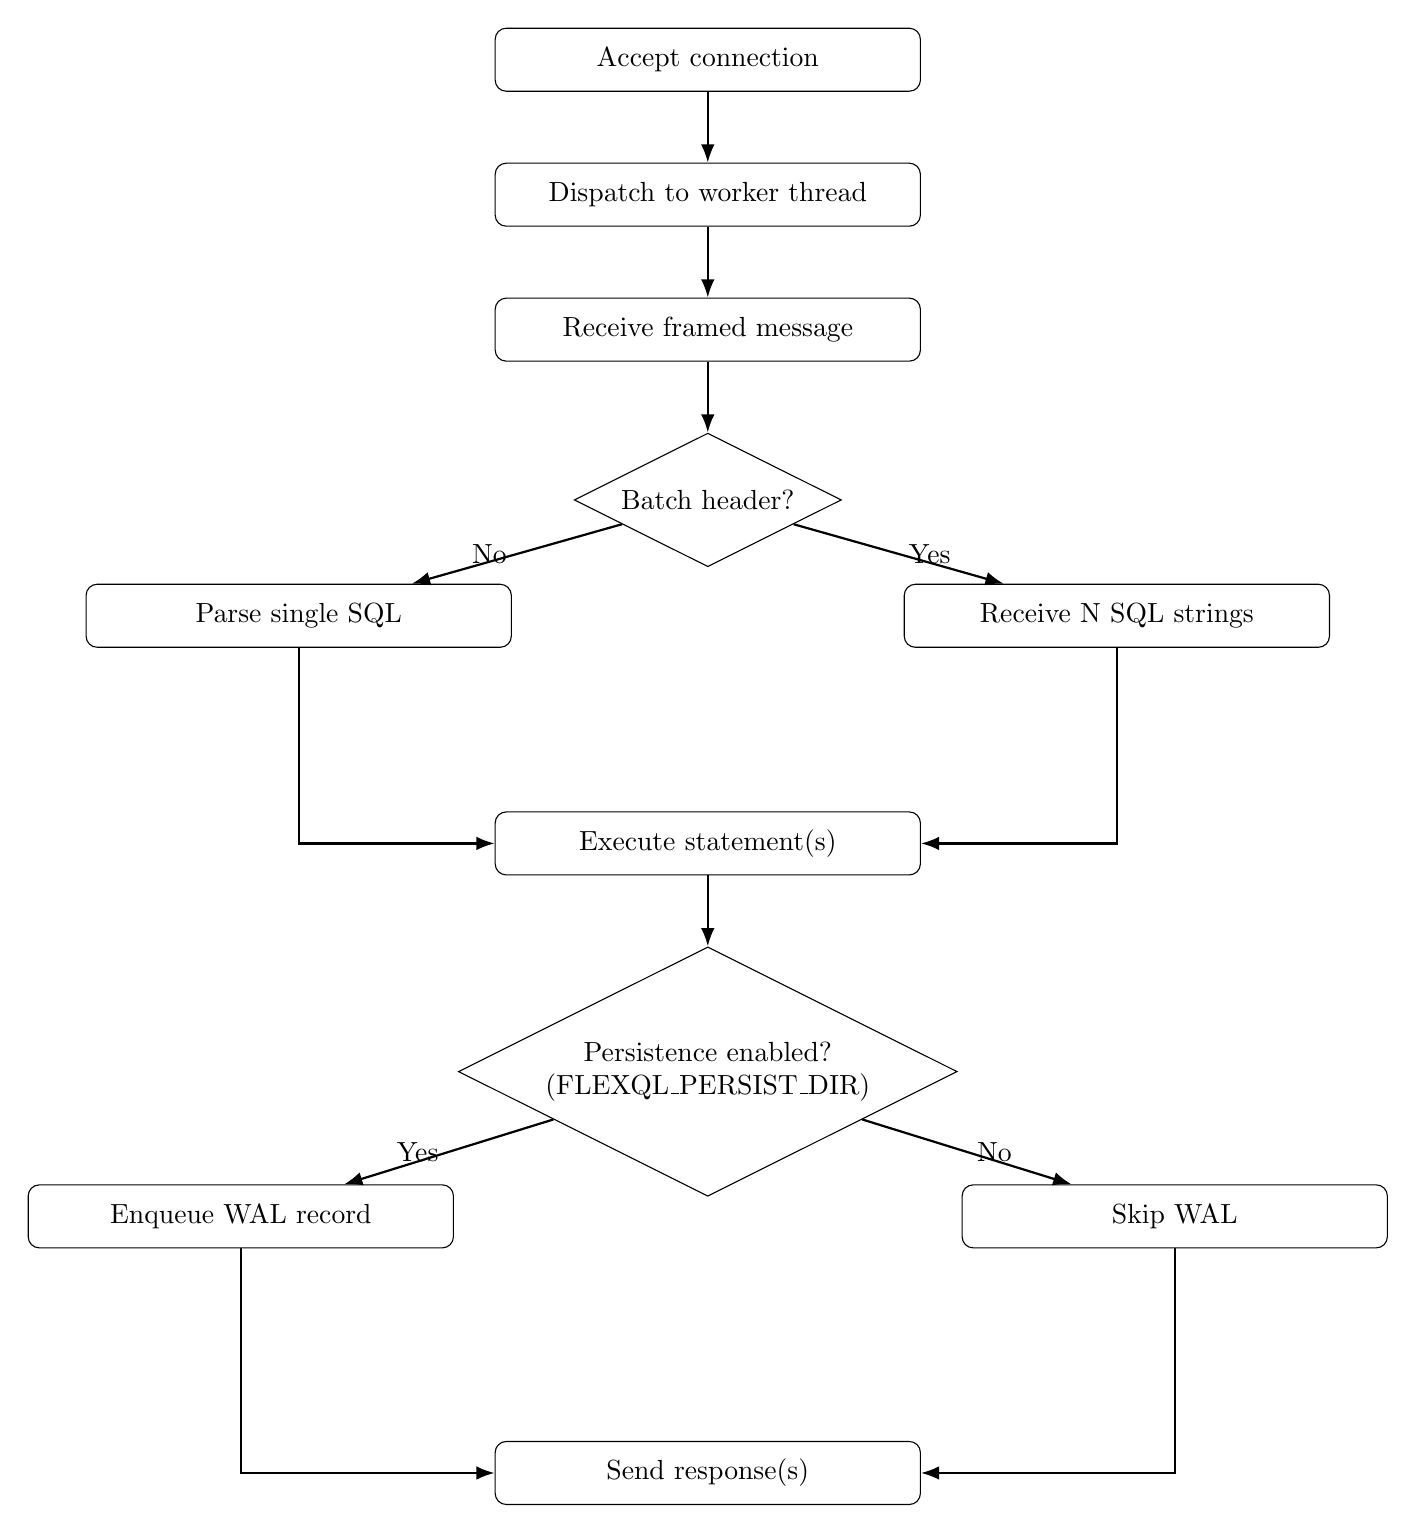
\begin{tikzpicture}[
  node distance=9mm,
  box/.style={rectangle,draw,rounded corners,align=center,minimum width=54mm,minimum height=8mm},
  decision/.style={shape=diamond,draw,align=center,aspect=2},
  arr/.style={-Latex,thick}
]
\node[box] (accept) {Accept connection};
\node[box,below=of accept] (dispatch) {Dispatch to worker thread};
\node[box,below=of dispatch] (recv) {Receive framed message};
\node[decision,below=of recv] (batch) {Batch header?};
\node[box,below left=of batch,xshift=-10mm] (single) {Parse single SQL};
\node[box,below right=of batch,xshift=10mm] (multi) {Receive N SQL strings};
\node[box,below=of batch,yshift=-22mm] (exec) {Execute statement(s)};
\node[decision,below=of exec] (persist) {Persistence enabled?\\(FLEXQL\_PERSIST\_DIR)};
\node[box,below left=of persist,xshift=-10mm] (enq) {Enqueue WAL record};
\node[box,below right=of persist,xshift=10mm] (skip) {Skip WAL};
\node[box,below=of persist,yshift=-22mm] (send) {Send response(s)};

\draw[arr] (accept) -- (dispatch);
\draw[arr] (dispatch) -- (recv);
\draw[arr] (recv) -- (batch);
\draw[arr] (batch) -- node[left]{No} (single);
\draw[arr] (batch) -- node[right]{Yes} (multi);
\draw[arr] (single) |- (exec);
\draw[arr] (multi) |- (exec);
\draw[arr] (exec) -- (persist);
\draw[arr] (persist) -- node[left]{Yes} (enq);
\draw[arr] (persist) -- node[right]{No} (skip);
\draw[arr] (enq) |- (send);
\draw[arr] (skip) |- (send);
\end{tikzpicture}

\caption{Request lifecycle (normal and batch modes)}
\end{figure}

\section{Storage Design}
\subsection{Row store}
Tables are stored in-memory using a row-major layout. Rows contain an array of field values (one per column), making INSERT and SELECT * simple and efficient for OLTP-style workloads.

\subsection{Arena allocation}
Instead of allocating each row with \texttt{malloc}, FlexQL allocates row memory from arena blocks to reduce allocator overhead and improve locality.

\subsection{TTL expiration}
Rows may include an optional expiration timestamp. A background sweeper thread periodically removes expired rows under per-table write locks.

\section{Indexing}
Primary key tables use an open-addressing hash index for O(1) average point lookups. The executor can use the index automatically for WHERE clauses targeting the primary key.

\section{LRU Query Cache}
FlexQL caches results of selected read queries using an LRU policy. Cached results are invalidated after successful inserts affecting a table.

\begin{figure}[H]
\centering
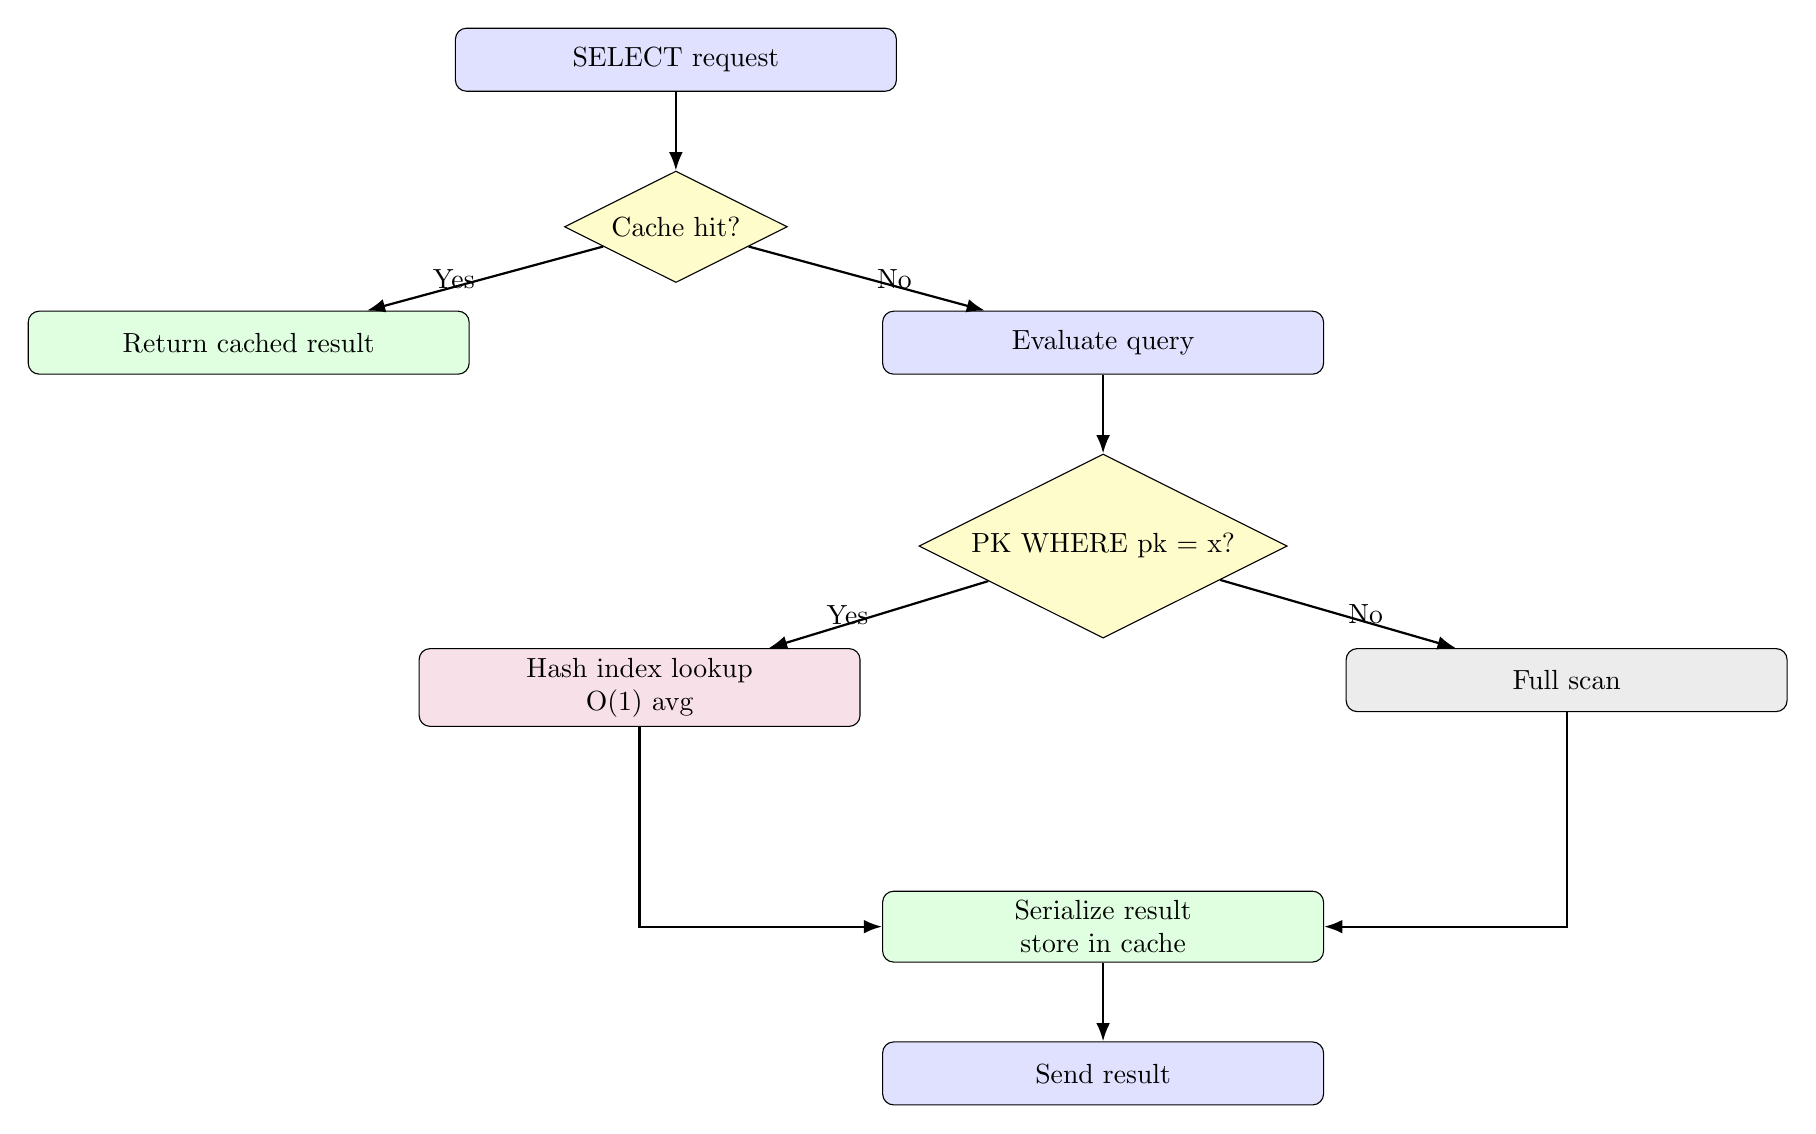
\begin{tikzpicture}[
  node distance=10mm,
  box/.style={rectangle,draw,rounded corners,align=center,minimum width=56mm,minimum height=8mm},
  decision/.style={shape=diamond,draw,align=center,aspect=2},
  arr/.style={-Latex,thick}
]
\node[box,fill=blue!12] (q) {SELECT request};
\node[decision,below=of q,fill=yellow!20] (hit) {Cache hit?};
\node[box,below left=of hit,xshift=-12mm,fill=green!12] (ret) {Return cached result};
\node[box,below right=of hit,xshift=12mm,fill=blue!12] (eval) {Evaluate query};
\node[decision,below=of eval,fill=yellow!20] (pk) {PK WHERE pk = x?};
\node[box,below left=of pk,xshift=-12mm,fill=purple!12] (idx) {Hash index lookup\\O(1) avg};
\node[box,below right=of pk,xshift=12mm,fill=gray!15] (scan) {Full scan};
\node[box,below=of pk,yshift=-22mm,fill=green!12] (store) {Serialize result\\store in cache};
\node[box,below=of store,fill=blue!12] (resp) {Send result};

\draw[arr] (q) -- (hit);
\draw[arr] (hit) -- node[left]{Yes} (ret);
\draw[arr] (hit) -- node[right]{No} (eval);
\draw[arr] (eval) -- (pk);
\draw[arr] (pk) -- node[left]{Yes} (idx);
\draw[arr] (pk) -- node[right]{No} (scan);
\draw[arr] (idx) |- (store);
\draw[arr] (scan) |- (store);
\draw[arr] (store) -- (resp);
\end{tikzpicture}

\caption{SELECT execution with cache and optional primary-key fast path}
\end{figure}

\section{Concurrency}
\subsection{Thread pool}
The server accepts connections on the main thread and dispatches each connection to a fixed worker pool:
\begin{center}
\texttt{THREAD\_POOL\_SZ = 32}
\end{center}

\subsection{Locking}
Read/write locks are used to allow multiple concurrent readers while ensuring correctness for inserts and expiry operations.

\begin{figure}[H]
\centering
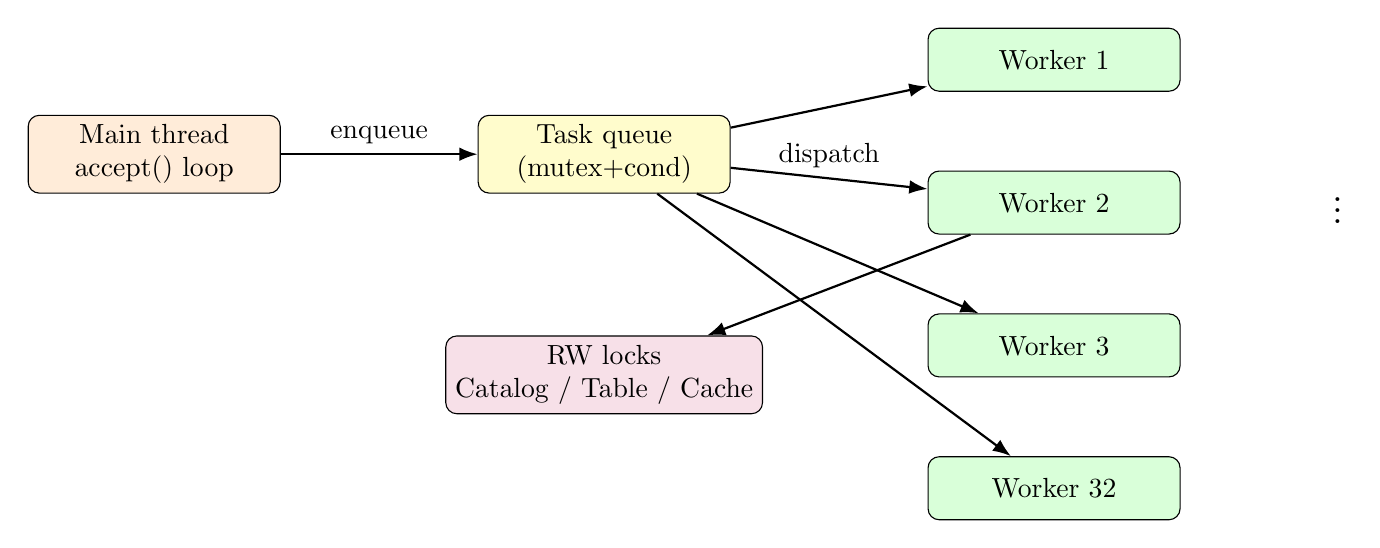
\begin{tikzpicture}[
  node distance=10mm,
  box/.style={rectangle,draw,rounded corners,align=center,minimum width=32mm,minimum height=8mm},
  arr/.style={-Latex,thick}
]
\node[box,fill=orange!15] (main) {Main thread\\accept() loop};
\node[box,fill=yellow!20,right=25mm of main] (queue) {Task queue\\(mutex+cond)};

\node[box,fill=green!15,right=25mm of queue,yshift=12mm] (w1) {Worker 1};
\node[box,fill=green!15,below=of w1] (w2) {Worker 2};
\node[box,fill=green!15,below=of w2] (w3) {Worker 3};
\node[right=18mm of w2] (dots) {\Large $\vdots$};
\node[box,fill=green!15,below=of w3] (wn) {Worker 32};

\node[box,fill=purple!12,below=18mm of queue] (locks) {RW locks\\Catalog / Table / Cache};

\draw[arr] (main) -- node[above]{enqueue} (queue);
\draw[arr] (queue) -- node[above]{dispatch} (w2);
\draw[arr] (queue) -- (w1);
\draw[arr] (queue) -- (w3);
\draw[arr] (queue) -- (wn);
\draw[arr] (w2) -- (locks);
\end{tikzpicture}

\caption{Concurrency model: accept loop + task queue + worker pool}
\end{figure}

\section{Persistence \& Fault Tolerance (WAL)}
\subsection{Enabling persistence}
Persistence is enabled via environment variable:\\
\begin{lstlisting}[language=bash]
mkdir -p ./persist
FLEXQL_PERSIST_DIR=./persist ./bin/flexql-server 9000
\end{lstlisting}
The WAL file is created at \texttt{./persist/flexql.wal}.

\subsection{WAL writer}
Mutations (CREATE TABLE / INSERT) are encoded and enqueued to a WAL queue protected by a mutex and condition variable. A dedicated background thread drains the queue and appends records to the WAL file.

\subsection{Recovery}
On startup with persistence enabled, the server replays WAL records to reconstruct the in-memory database state.

\begin{figure}[H]
\centering
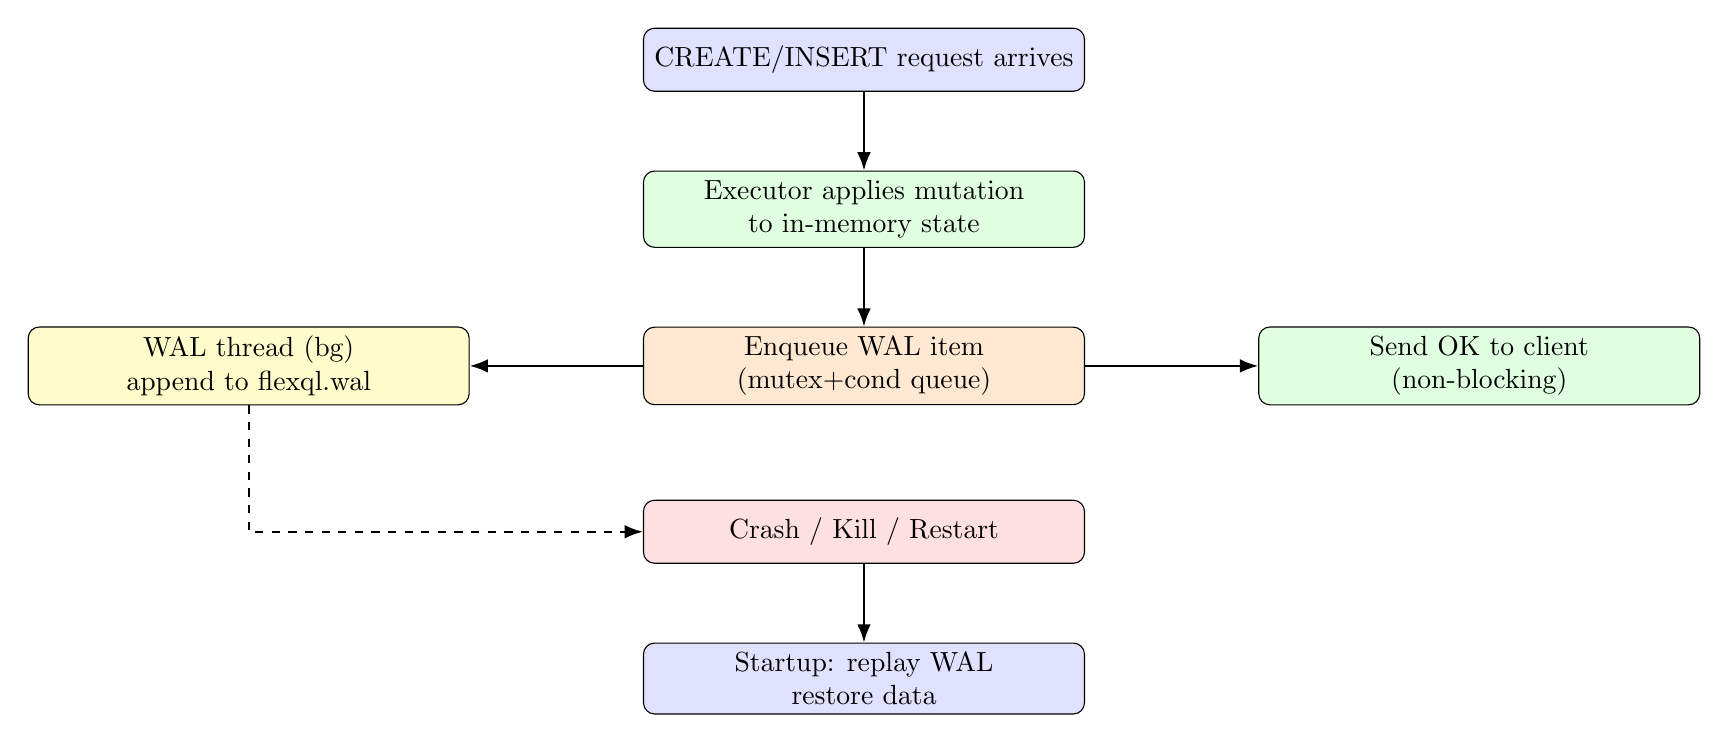
\begin{tikzpicture}[
  node distance=10mm,
  box/.style={rectangle,draw,rounded corners,align=center,minimum width=56mm,minimum height=8mm},
  arr/.style={-Latex,thick}
]
\node[box,fill=blue!12] (stmt) {CREATE/INSERT request arrives};
\node[box,fill=green!12,below=of stmt] (exec) {Executor applies mutation\\to in-memory state};
\node[box,fill=orange!18,below=of exec] (enq) {Enqueue WAL item\\(mutex+cond queue)};
\node[box,fill=yellow!20,left=22mm of enq] (wal) {WAL thread (bg)\\append to flexql.wal};
\node[box,fill=green!12,right=22mm of enq] (ok) {Send OK to client\\(non-blocking)};
\node[box,fill=red!12,below=12mm of enq] (crash) {Crash / Kill / Restart};
\node[box,fill=blue!12,below=of crash] (replay) {Startup: replay WAL\\restore data};

\draw[arr] (stmt) -- (exec);
\draw[arr] (exec) -- (enq);
\draw[arr] (enq) -- (wal);
\draw[arr] (enq) -- (ok);
\draw[arr] (crash) -- (replay);
\draw[arr,dashed] (wal) |- (crash);
\end{tikzpicture}

\caption{WAL write and recovery flow}
\end{figure}

\section{High-Performance Batch INSERT}
Large insert workloads are accelerated by combining:
\begin{itemize}
  \item Multi-row INSERT syntax (one statement contains many tuples)
  \item Batch protocol (send many SQL strings in one round trip)
\end{itemize}

\begin{figure}[H]
\centering
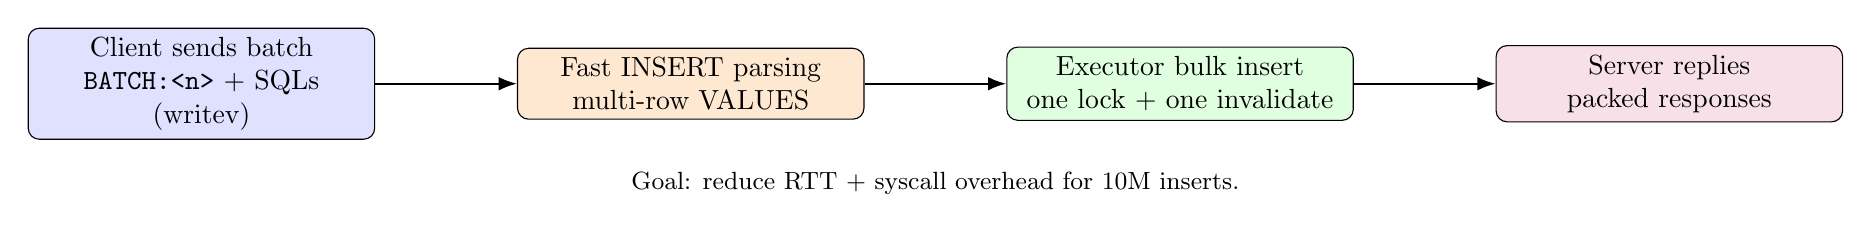
\begin{tikzpicture}[
  box/.style={rectangle,draw,rounded corners,align=center,minimum width=44mm,minimum height=9mm},
  arr/.style={-Latex,thick}
]
\node[box,fill=blue!12] (c) {Client sends batch\\\texttt{BATCH:<n>} + SQLs\\(writev)};
\node[box,fill=orange!18,right=18mm of c] (p) {Fast INSERT parsing\\multi-row VALUES};
\node[box,fill=green!12,right=18mm of p] (e) {Executor bulk insert\\one lock + one invalidate};
\node[box,fill=purple!12,right=18mm of e] (r) {Server replies\\packed responses};

\draw[arr] (c) -- (p);
\draw[arr] (p) -- (e);
\draw[arr] (e) -- (r);

\node[below=10mm of $(p)!0.5!(e)$] (note) {\small Goal: reduce RTT + syscall overhead for 10M inserts.};
\end{tikzpicture}

\caption{High-performance batch insert path}
\end{figure}

\section{Supported SQL Subset}
Supported:
\begin{itemize}
  \item \texttt{CREATE TABLE}
  \item \texttt{INSERT INTO ... VALUES (...)} and multi-row \texttt{VALUES (...),(...),...}
  \item \texttt{SELECT} with single-condition WHERE operators: \texttt{=, <, >, <=, >=}
  \item \texttt{INNER JOIN} (as implemented)
\end{itemize}
Not supported:
\begin{itemize}
  \item \texttt{SHOW TABLES} / \texttt{SHOW DATABASES}
  \item \texttt{UPDATE} / \texttt{DELETE}
\end{itemize}

\section{Build \& Run (Commands)}
\subsection{Build}
\begin{lstlisting}[language=bash]
make clean
make -j
\end{lstlisting}

\subsection{Run server (in-memory)}
\begin{lstlisting}[language=bash]
FLEXQL_NO_EXPIRY=1 ./bin/flexql-server 9000
\end{lstlisting}

\subsection{Run server (with persistence)}
\begin{lstlisting}[language=bash]
mkdir -p ./persist
FLEXQL_PERSIST_DIR=./persist FLEXQL_NO_EXPIRY=1 ./bin/flexql-server 9000
\end{lstlisting}

\subsection{Run REPL}
\begin{lstlisting}[language=bash]
./bin/flexql-client 127.0.0.1 9000
\end{lstlisting}

REPL meta-commands supported: \texttt{.help}, \texttt{.clear}, \texttt{.exit/.quit}.

\subsection{Run bundled C benchmark}
\begin{lstlisting}[language=bash]
./bin/flexql-bench 127.0.0.1 9000 10000000
\end{lstlisting}

\subsection{Run official C++ benchmark (benchmark\_flexql.cpp)}
Compile the benchmark file as C++ and link against the FlexQL C client library:\\
\begin{lstlisting}[language=bash]
# Terminal 1
kill -9 $(pidof flexql-server) 2>/dev/null || true
FLEXQL_NO_EXPIRY=1 ./bin/flexql-server 9000

# Terminal 2
g++ -O3 -march=native -std=c++17 -Iinclude benchmark_flexql.cpp bin/libflexql.a -lpthread -o bin/benchmark_flexql_cpp
./bin/benchmark_flexql_cpp --unit-test
./bin/benchmark_flexql_cpp 10000000
\end{lstlisting}

Note: run on a fresh server. Re-running without restarting may fail with \texttt{Table already exists} and show duplicated rows.

\section{Testing Checklist (Manual)}
\begin{itemize}
  \item Correctness: create table, insert, select, where operators
  \item Concurrency: open multiple clients and perform parallel inserts/selects
  \item Persistence: enable WAL, insert data, kill server, restart, verify data
  \item Fault tolerance: invalid SQL returns error and server stays alive
  \item Benchmark: run 1M then 10M insert benchmark
\end{itemize}

\section{Limitations and Future Work}
\begin{itemize}
  \item Add catalog queries (e.g., list tables)
  \item Improve WAL durability guarantees (fsync policy)
  \item Extend WHERE support (AND/OR), add UPDATE/DELETE
  \item Add more robust query planning and join strategies
\end{itemize}

\end{document}
